\documentclass[11pt,a4paper]{article}
\usepackage[utf8]{inputenc}\usepackage[T1]{fontenc}
\usepackage[margin=1in]{geometry}
\usepackage{amsmath,amssymb,booktabs,array,graphicx,enumitem,xcolor,parskip,titlesec}
\usepackage[hidelinks]{hyperref}
\graphicspath{{figures/}}
\definecolor{qnavy}{RGB}{20,40,75}\definecolor{qgrey}{RGB}{90,90,90}\definecolor{qred}{RGB}{150,30,30}
\titleformat{\section}{\large\bfseries\color{qnavy}}{\thesection}{0.6em}{}
\input{MACROS.tex}
\emergencystretch=2em
\begin{document}\thispagestyle{empty}
\noindent
{\large\bfseries\color{qnavy} Report R14 --- Autonomous Analysis Generation on a Sealed Cohort}\\[2pt]
{\color{qgrey}Arm A, exposure 1: a generator agent, given a never-seen multimodal ICI cohort
(Vanguri et al., MSK), pre-registered and executed a complete gate-carrying analysis with zero
human pipeline edits --- and returned a calibrated null on the question the cohort cannot
answer.}\\[6pt]
{\color{qgrey}\rule{\textwidth}{0.4pt}}

\medskip
\noindent 11 August 2026 \quad\textbullet\quad Quantara \quad\textbullet\quad
NSCLC RWPR study, Arm A

\section*{Summary}

Arm A tests the study's core claim: \emph{a system exposed to a dataset it has never seen must
produce a valid, pre-registered, executable analysis --- and must refuse to manufacture findings
the data cannot support.} The sealed cohort was the study's premier holdout: 247 stage-IV NSCLC
patients treated with anti-PD-(L)1 (RECIST~1.1 response, OS/PFS, PD-L1 IHC slides, MSK-IMPACT
panel, CT radiomics). The generator saw only object listings and public cohort facts before
hashing its analysis plan; the original authors' analysis code was placed under a self-imposed,
auditable firewall for the entire arm. Every number here is extracted mechanically from the
evidence bundle by \texttt{extract\_numbers.py}.

\textbf{What worked:} the clinical + PD-L1 + TMB/genomic baseline predicts response at
\textbf{AUROC \RBaseAuroc} (\RBaseLo--\RBaseHi; $n=\RBaseN$; Holm-corrected permutation
$p=\RBaseHolm$) and OS at \textbf{C-index \ROsBaseC} (\ROsBaseLo--\ROsBaseHi;
$p=\ROsBaseP$). \textbf{What the system refused to claim:} the pre-registered primary hypothesis
--- that the full multimodal stack beats that baseline --- returned
\textbf{\RVerdict}: at the $n=\RHOneN$ all-modality intersection the paired
$\Delta$AUROC is \RHOneDelta{} (CI \RHOneDeltaLo{} to \RHOneDeltaHi, one-sided
$p=\RHOneP$), with a bootstrap CI half-width of \RHOneHalfwidth{} against the pre-declared
0.06 sensitivity bar --- and \emph{every} modality-addition delta is $\leq 0$. The null was
pre-declared as a success mode before any label was read; delivering it, rather than a
manufactured positive, is the central claim of this report.

\textbf{One well-controlled novel observation}: Phikon-v2, an H\&E foundation model, reads
PD-L1 IHC slides zero-shot --- its embeddings predict TPS\,$\geq$\,50\% at
\textbf{AUROC \RPcThreeAuroc} (\RPcThreeLo--\RPcThreeHi, $n=\RPcThreeN$). One positive
control (RECIST target-lesion volume $\rightarrow$ OS) \textbf{failed its expectation}; the
failure is adjudicated in \S4 as a genuine cohort-level null, retained rather than deleted.

\section{What Arm A tests}

The contract (\texttt{evidence/config.yaml}, PROTOCOL \S4): the generator receives only the
sealed dataset's file listing, a data dictionary's worth of public facts, and the standing gate
library. It must produce a pre-registered config (hashed before labels are read), an executable
pipeline, and the full R-series evidence bundle; the human role is to run it, not edit it.
Success is defined by execution + gates + calibrated claims, explicitly \emph{including} a
null or inconclusive verdict on an underpowered endpoint. Endpoints and the primary hypothesis
(multimodal $>$ clinical baseline, paired, one-sided) were fixed in the config; so were the
verdict rules that computed the \RVerdict{} outcome mechanically.

\section{The integrity chain}

\begin{itemize}[leftmargin=1.2em,itemsep=2pt]
\item \textbf{2026-08-10T23:39:01Z} --- config written and SHA-256-hashed
(\texttt{\RConfigShaShort}\ldots), mirrored to GCS. Declared pre-hash reads: object
name/size listings and public cohort facts only --- \emph{no sealed file content and no column
headers} (stricter than Arm B's event \#1).
\item \textbf{2026-08-10T23:39:35Z} --- unsealing event \#3 appended to the remote append-only
log with a GCS generation precondition, carrying the config hash.
\item \textbf{2026-08-10T23:43Z} --- first sealed content staged (local mtimes + GCS audit),
i.e.\ strictly after the hash and the event (gate G1).
\item \textbf{Contamination firewall.} The authors' own analysis code and permutation outputs
(\texttt{code/**}, \texttt{tests/**}) were declared off-limits for the whole arm --- reading
them would contaminate the autonomy claim. Gate G11 attests zero reads: the executed pipeline
contains no reference to those prefixes, and \texttt{inputs.json} enumerates (with SHA-256)
all 16 staged sealed files, none from them. The authors' released \emph{feature tables} are
declared inputs, not analysis code.
\item \textbf{Schema by rule, not by peeking.} Because no header was read pre-hash, column
mapping was pre-registered as an ordered regex ruleset; the executed mapping and every
mapping decision is dumped to \texttt{evidence/schema\_map.json}.
\end{itemize}

\section{Results}

\begin{center}
\small
\input{generated_e1_table}
\end{center}
\noindent{\small\color{qgrey}E1 = RECIST~1.1 best overall response (CR/PR vs SD/PD), repeated
stratified 5-fold CV $\times$ 5 seeds, all preprocessing inside folds; AUROC of the mean
out-of-fold prediction. MDE = minimum detectable AUROC at 80\% power. Holm correction across
the 6-model family; bold = significant. Permutation nulls are full-CV refits (1{,}000 per
model), all centred at 0.5 (gate G7).}

\begin{center}
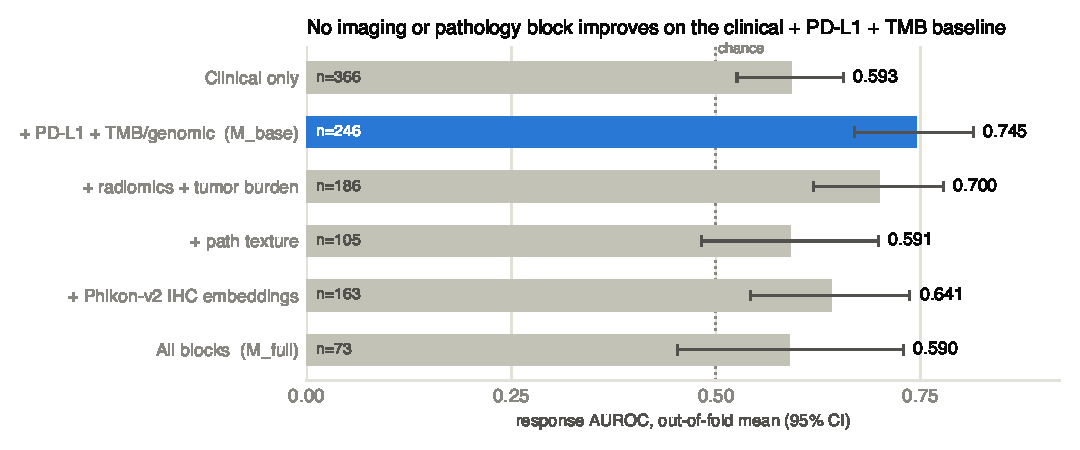
\includegraphics[width=0.94\textwidth]{fig_modalities.pdf}
\end{center}

\textbf{The primary hypothesis, exactly as adjudicated.} H1 compared M\_full vs M\_base paired
on the identical patients and folds (fold-subset hash \texttt{\RFoldHash}), $n=\RHOneN$
(\RHOnePos{} responders): $\Delta$AUROC $= \RHOneDelta$ (\RHOneDeltaLo{} to \RHOneDeltaHi),
one-sided $p=\RHOneP$. The pre-declared rule says: if the delta CI half-width implies an MDE
above 0.06, the verdict is power-limited regardless of $p$ --- observed half-width
\RHOneHalfwidth, three times that bar. Verdict: \textbf{\RVerdict}. The direction is
consistent everywhere: adding radiomics ($\RDeltaRad$), path texture ($\RDeltaPathg$), or IHC
embeddings ($\RDeltaPathf$) to the baseline never helps on the paired subsets, and on OS the
full stack is significantly \emph{worse} ($\Delta$C $= \RHThreeDelta$, CI \RHThreeDeltaLo{}
to \RHThreeDeltaHi) --- at $n=\RHOneN$ the extra blocks are noise the model must overfit.

\begin{center}
\small
\input{generated_e2_table}
\end{center}
\noindent{\small\color{qgrey}E2 = overall survival (Cox, out-of-fold risk); permutation nulls
(500 refits) were pre-registered for M\_base and M\_full only. PFS (E3) was descriptive:
M\_base C 0.665, M\_full 0.458 --- same pattern.}

\textbf{The honest summary a partner should take away:} on this cohort, response is best
predicted by the boring model --- clinical covariates + PD-L1 TPS + TMB/genomics at
\RBaseAuroc{} --- and the value of imaging and pathology \emph{cannot be adjudicated} at the
$n=\RHOneN$ patients who carry every modality. That is a statement about cohort intersection
size, not about imaging; it is exactly the gap a larger linked cohort closes.

\section{Positive controls and gates}

PC1 (PD-L1 TPS alone $\rightarrow$ response): AUROC \RPcOneAuroc, $p=\RPcOneP$ --- label join
and endpoint coding proven. PC3 (competence of the IHC encoding): \RPcThreeAuroc{}
(\RPcThreeLo--\RPcThreeHi) --- see \S5. PC4 (join integrity): \RPcFourJoin{} clinical-genomic
joins, sex agreement \RPcFourSex\%.

\textbf{PC2 failed, and the failure is informative.} Seg-derived baseline tumor volume did not
predict OS (C \RPcTwoC, HR/SD \RPcTwoHr, $p=\RPcTwoP$; $n=\RPcTwoN$, \RPcTwoEvents{} events).
The adjudication, verbatim from \texttt{gates.json}: \emph{``\input{generated_g3_adjudication}''}
The gate row is retained as FAIL rather than reclassified; per the pre-registered verdict
rules it participates only in H1 \emph{confirmation}, and H1 is a null regardless.

\begin{center}
\footnotesize
\input{generated_gates_table}
\end{center}
\noindent{\small\color{qgrey}\RNGatesPass{} of \RNGates{} gates pass; G3 is the adjudicated
failure above. Budget (G9): total compute $<$\,\$5 on Modal (234 L4 slide-encoding tasks
$\approx$ 1.2 GPU-hours) plus local CPU.}

\section{The novel observation: an H\&E foundation model reads IHC}

PC3 was designed as a competence control and returned more than competence: Phikon-v2
embeddings of the PD-L1 IHC slides --- an encoder trained on H\&E histology, applied zero-shot
to a different stain --- predict TPS\,$\geq$\,50\% at \textbf{AUROC \RPcThreeAuroc}
(\RPcThreeLo--\RPcThreeHi; $n=\RPcThreeN$, \RPcThreePos{} positive), under the same
leakage-controlled CV as everything else. The control is well-posed because the label (TPS) is
scored by pathologists from these very slides, so this is signal recovery, not prognosis ---
and for the same reason it is \emph{not} a clinical claim. What it does establish: the slide
representation carried real information (the response nulls above are not ``the encoder saw
nothing''), and IHC quantification from foundation-model embeddings is a measurable,
well-controlled capability the original publication did not test (the authors used
hand-crafted texture features on these slides).

\section{Limitations --- the skeptic's list}

No separate limitations memo exists in the evidence bundle; this section is assembled
\emph{verbatim} from the self-critical statements the generator recorded inside its
pre-registered config and evidence files, each quoted with its source, plus three points
from the generator's final self-assessment, which existed only in its closing report and
is archived unedited at \texttt{nsclc-rwpr-study/armA/GENERATOR\_SELF\_ASSESSMENT.md}.
Nothing is softened.

\begin{itemize}[leftmargin=1.2em,itemsep=2pt]
\item \textbf{Power was predicted to be the binding constraint --- before unsealing}
(\texttt{config.yaml power.honesty}): \emph{``expected regime: n$\approx$247, $\sim$25--40\%
responders $\rightarrow$ single-model MDE $\approx$ 0.60--0.62 AUROC; delta-AUROC below
$\sim$0.06--0.08 is likely undetectable. A null on H1 with this statement is a SUCCESS
outcome.''} The realized intersection ($n=\RHOneN$) was far worse than that forecast.
\item \textbf{The H1 comparison is three times less sensitive than its own bar}
(\texttt{results.json H1.delta\_mde\_note}): \emph{``bootstrap delta CI half-width =
0.1854''} against the pre-declared 0.06 rule.
\item \textbf{Modality attrition biases the intersection}: availability falls
\RAvClin{} (clinical) $\rightarrow$ \RAvPdl{} (PD-L1) $\rightarrow$ \RAvRad{} (radiomics)
$\rightarrow$ \RAvPathg{} (path texture) $\rightarrow$ \RHOneN{} (all blocks); the
complete-case subset is whoever happened to get every assay, not a random sample.
\item \textbf{A positive control failed} (G3, quoted in full in \S4): RECIST target-lesion
volume did not predict OS. Adjudicated as a genuine cohort-level null with competence
separately established --- but a failed control is a failed control, and it is retained as
FAIL.
\item \textbf{OS exists only for the discovery cohort}
(\texttt{schema\_map.json}): \emph{``OS available for 246 patients (msk\_mind discovery only:
censored follow-up time absent from patient\_listing)''} --- 120 patients are logged
exclusions on E2.
\item \textbf{Two intended clinical covariates never materialized}
(\texttt{schema\_map.json}): the pre-registered patterns for histology and line-of-therapy
\emph{``matched no column''} --- the clinical block is thinner than designed.
\item \textbf{The radiomics signal is fragile out-of-split}
(\texttt{sensitivity.json S2}): on the authors' own train/validation split, the
radiomics-block model scores \RAuthorSplitRad{} (\RAuthorSplitRadLo--\RAuthorSplitRadHi) on
the held-out validation rows --- consistent with chance.
\item \textbf{Single institution, single cohort}: every estimate above is MSK-internal
cross-validation; no external cohort exists for these endpoints in the sealed pool.
\item \textbf{The intersection is confounded, not just small}
(archived self-assessment): modality availability tracks cohort membership (discovery
vs.\ validation), so the all-modality subset is structurally biased --- in the
generator's own words, \emph{``a stronger design would have pre-registered the pairwise
intersections as primary.''}
\item \textbf{The permutation statistic is not the headline statistic}
(archived self-assessment): permutation nulls refit the seed-0 cross-validated AUROC
while the headline is the 5-repeat mean; \texttt{results.json} documents both and the
values are nearly identical, but the mismatch is real.
\item \textbf{Two block-construction choices could bias modality conclusions}
(archived self-assessment): the PD-L1 block mixes Sauter re-scores with clinical scores
(45 fallback fills, logged), and the pathology foundation-model block uses mean-pooling
rather than attention-MIL --- a weak pooling choice that could understate the pathology
signal H1 concluded nothing about.
\end{itemize}

\section{Protocol status}

Protocol success criterion \#1 requires \emph{``$\geq$2 sealed holdouts processed with zero
human pipeline edits; all evidence bundles complete; no gate-failing claim shipped.''}
\textbf{This report is exposure 1 of that bar} --- the criterion is not yet met, and no claim
that it is met is made here. Arm B-meth's unsealing (event \#2, R13) was a model-transfer
exposure, not an Arm A generation. The remaining sealed holdouts (anti-PD-1 EPIC arrays are
consumed; ACRIN PET, LUSC imaging mass spec, Anti-PD-1-Lung imaging remain) are the candidates
for exposure 2.

\section{Reproducing this report}

\begin{itemize}[leftmargin=1.2em,itemsep=1pt]
\item Every number: \texttt{python3 extract\_numbers.py}; figure:
\texttt{python3 make\_figures.py}. Evidence: verbatim copy of
\texttt{nsclc-rwpr-study/armA/evidence/} (run of 2026-08-11, 30 files), plus
\texttt{config.yaml}, whose SHA-256 equals the \texttt{config\_sha256} inside
\texttt{results.json}.
\item Any AUROC can be recomputed from the out-of-fold files, e.g.\ the headline:
\begin{quote}\small\begin{verbatim}
python3 -c "
import pandas as pd; from sklearn.metrics import roc_auc_score
d=pd.read_csv('evidence/oof_e1_M_base.csv')
print(roc_auc_score(d['label'], d['pred_mean']))"   # -> 0.7448
\end{verbatim}\end{quote}
\item Pipeline code as executed: \texttt{nsclc-rwpr-study/armA/\{build\_dataset, run\_analysis,
run\_sensitivity, finalize\_evidence\}.py} (mirrored to GCS with the evidence).
\item Unsealing event \#3: the remote append-only log in the study bucket under\\
\texttt{nsclc-rwpr-study/\_provenance/}.
\end{itemize}

\end{document}
